\chapter{Experimental Setup}
\label{ch:setup}

We formalize the distillation problem as follows.
A teacher policy $\pi_T$ is trained via RL on a fully-observable MDP $\mathcal{M} = (\mathcal{S}, \mathcal{A}, T, R, \gamma)$.
At deployment, the student observes only a partial view $o_t = \phi(s_t)$ of the true state, yielding a POMDP.
The student $\pi_S$ is trained to minimize behavioral cloning loss over teacher demonstrations $\mathcal{D} = \{(o_{1:T}^{(i)}, a_{1:T}^{(i)})\}_{i=1}^N$:
\begin{equation}
  \pi_S^* = \arg\min_{\pi_S} \sum_{i=1}^N \sum_{t=1}^{T_i} \| \pi_S(o_{1:t}^{(i)}) - a_t^{(i)} \|^2
  \label{eq:bc}
\end{equation}
The student must map observation \emph{sequences} to actions because a single observation $o_t$ is insufficient to recover the hidden state components (e.g., velocities).
This makes the choice of temporal backbone---how the student processes the sequence $o_{1:t}$---the central design decision we study.

\section{Student Architectures}
\label{sec:architectures}

We compare four temporal backbones plus two non-temporal baselines.
All share input projection ($\text{obs\_dim} \to d_\text{model}$) and output projection ($d_\text{model} \to \text{act\_dim}$); only the temporal backbone differs.
Default: $d_\text{model} = 64$, 2 layers.

\paragraph{GRU} (Gated Recurrent Unit~\citep{cho2014gru}).
Maintains hidden state $h_t \in \R^{d}$ via learned reset and update gates:
\begin{align}
  z_t &= \sigma(W_z x_t + U_z h_{t-1}) & \text{(update gate)} \\
  r_t &= \sigma(W_r x_t + U_r h_{t-1}) & \text{(reset gate)} \\
  h_t &= (1 - z_t) \odot h_{t-1} + z_t \odot \tanh(W_h x_t + U_h (r_t \odot h_{t-1}))
\end{align}
The strongest baseline on the POPGym memory benchmark~\citep{morad2023popgym}, and the simplest of our temporal architectures. Parameters: $\sim$51K.

\paragraph{LSTM} (Long Short-Term Memory~\citep{hochreiter1997lstm}).
Adds a cell state $c_t$ alongside $h_t$, with forget, input, and output gates.
The additional cell state provides a ``highway'' for gradient flow and a mechanism for selective information retention via the forget gate.
Same architecture family as our teacher (RecurrentPPO uses LSTM internally).
Parameters: $\sim$68K.

\paragraph{Transformer.}
Causal self-attention with a sliding window of 64 steps (chosen to match the typical velocity-inference horizon in our MuJoCo POMDPs; a larger window would solve T-Maze at $L{=}200$ but at quadratic attention cost), 4 heads, pre-norm residual blocks.
Attention provides \emph{content-addressable} memory: the model can directly query past observations by content similarity rather than compressing them into a fixed-size state.
The sliding window limits the context to the most recent 64 observations, which is sufficient for velocity inference but insufficient for T-Maze corridors longer than 64 steps.
Parameters: $\sim$232K.

\paragraph{STU} (Spectral Transform Unit~\citep{agarwal2024spectral, liu2025flashstu}).
Rather than learning temporal dynamics, STU uses \emph{fixed} spectral filters derived from the eigendecomposition of a Hankel matrix.
The Hankel matrix $Z \in \R^{L \times L}$ with entries $Z_{ij} = \frac{2}{(i+j)^3 - (i+j)}$ has the property that its top-$K$ eigenvectors $\{\phi_k\}_{k=1}^K$ form a universal basis for the impulse responses of causal linear dynamical systems~\citep{agarwal2024spectral}.
The STU output at each layer is:
\begin{equation}
  y_t = \sum_{k=1}^{K} \left( M_k^{+} \cdot (\phi_k * u)_t + M_k^{-} \cdot (\tilde{\phi}_k * u)_t \right) + W u_t
  \label{eq:stu}
\end{equation}
where $\phi_k * u$ denotes causal convolution of input $u$ with filter $\phi_k$ (computed via FFT), $\tilde{\phi}_k$ are sign-alternated filters, $M_k^{\pm}$ are learned projection matrices, and $W$ is a direct linear bypass.
The filters $\phi_k$ are fixed; only $M_k^{\pm}$ and $W$ are learned, making training convex in the parameters (Theorem~3.1 of~\citet{agarwal2024spectral}).
We use the \emph{full} STU (not the tensordot approximation STU-T), which catastrophically fails at small scale (\cref{sec:stu-t-failure}).
Parameters: $\sim$338K with $K=16$ filters.

\paragraph{GRU (parameter-matched).}
To disentangle architecture from capacity, we also test GRU at $d_\text{model} = 160$, producing $\sim$312K parameters---closely matching STU's 338K.
If GRU$_{160}$ still outperforms or matches STU, the advantage is architectural, not capacity-driven.

\paragraph{Baselines.}
An \textbf{MLP} (5K params) processes each timestep independently with no temporal context.
A \textbf{FrameStack} model (9K params) concatenates the 8 most recent observations and feeds them through an MLP---a generous window for finite-difference velocity estimation (which requires only $k{=}2$), meaning that if FrameStack still fails, the task genuinely requires learned temporal integration.

\begin{table}[ht]
\centering
\caption{Student architecture summary (HalfCheetah-POMDP; parameter counts vary with obs/act dimensions). All temporal models at $d_\text{model}=64$, 2 layers. Latency: single-step CPU inference on Apple M2 Max.}
\label{tab:arch-summary}
\begin{tabular}{lrrrl}
\toprule
Architecture & Params & Latency (ms) & Throughput (steps/s) & Key property \\
\midrule
MLP             &   5K & 0.1 & 10{,}000 & No temporal context \\
FrameStack ($k{=}8$) &  9K & 0.2 & 5{,}000 & Fixed-window history \\
GRU             &  51K & 1.26 & 796 & Learned gating, simplest \\
LSTM            &  68K & 1.33 & 751 & Learned gating + cell state \\
Transformer     & 232K & 3.36 & 297 & Content-addressable attention \\
STU (full)      & 338K & 4.38 & 228 & Fixed spectral filters, convex \\
\midrule
GRU$_{160}$ (param-matched) & 312K & 2.8 & 357 & Capacity-matched to STU \\
\bottomrule
\end{tabular}
\end{table}

Note the $6.6\times$ parameter gap between the smallest temporal student (GRU, 51K) and the largest (STU, 338K).
The parameter-matched GRU$_{160}$ addresses this confound directly.

\section{Tasks}
\label{sec:tasks}

We evaluate on two task families: synthetic controlled benchmarks with \emph{optimal} teachers and continuous-control POMDPs with \emph{learned} (imperfect) teachers.

\subsection{Synthetic Benchmarks (Optimal Teachers)}

These tasks use hand-coded optimal policies as teachers, eliminating teacher quality as a variable.

\paragraph{T-Maze.}
At step~0, the agent receives a directional hint (LEFT or RIGHT).
It traverses a corridor for $L$ steps observing only uninformative tokens.
At the end, it must choose the direction matching the hint (\cref{fig:task-diagrams}, top).
We test $L \in \{10, 50, 100, 200\}$. Maximum return ${=}1$; random ${=}0$.

\paragraph{CopyTask.}
The agent observes $N$ random tokens from vocabulary $V=8$, then must replay them in order (\cref{fig:task-diagrams}, bottom).
We test $N \in \{5, 10, 20\}$. Maximum return ${=}N$; random ${\approx} N/V$.

\begin{figure}[ht]
\centering
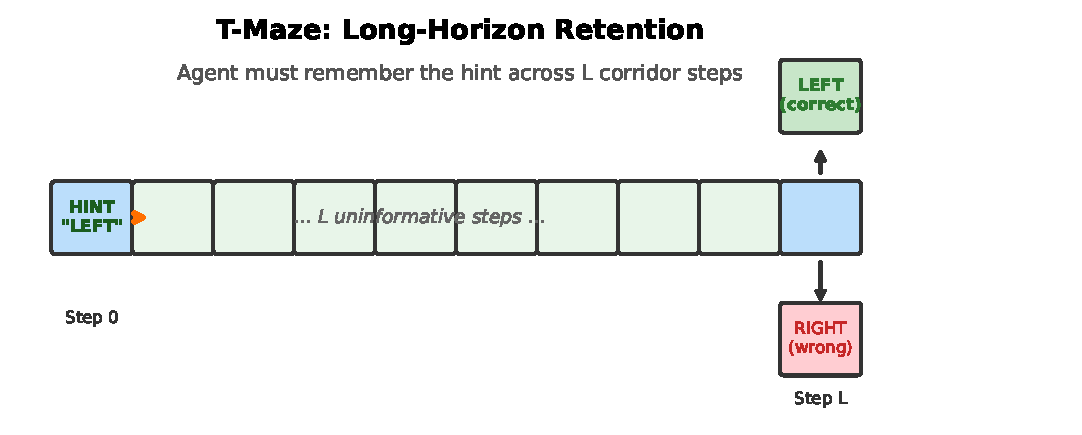
\includegraphics[width=0.85\textwidth]{diagram_tmaze.pdf}\\[2pt]
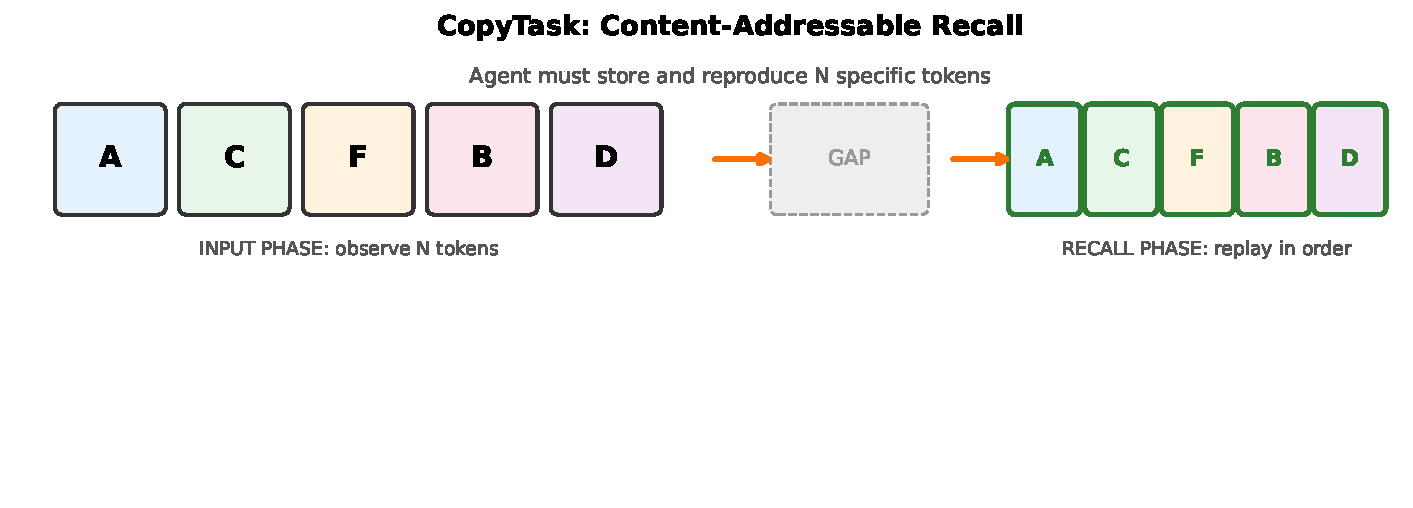
\includegraphics[width=0.85\textwidth]{diagram_copytask.pdf}
\caption{Synthetic benchmark tasks. \textbf{Top:} T-Maze --- the agent receives a hint at step~0, traverses $L$ uninformative steps, and must choose the matching direction. Tests long-horizon retention. \textbf{Bottom:} CopyTask --- the agent observes $N$ tokens, waits, then replays them in order. Tests content-addressable recall.}
\label{fig:task-diagrams}
\end{figure}

\subsection{MuJoCo POMDPs (Imperfect Teachers)}
\label{sec:mujoco-setup}

We create POMDPs from standard MuJoCo locomotion environments by removing velocity observations.
The agent observes only joint positions and must infer velocities from position history.

\paragraph{HalfCheetah-POMDP.} 8-dim positions (from 17-dim full obs), 6-dim actions.
\paragraph{Ant-POMDP.} 13-dim positions (from 27-dim), 8-dim actions.

\paragraph{MetaDrive.}
MetaDrive is an autonomous driving simulator with lidar-based observations (91-dim: 19 state dimensions + 72 lidar lasers at 50m range) and 2-dim continuous actions (steering, acceleration).
Unlike the MuJoCo POMDPs, MetaDrive is \emph{inherently} partially observable---no observation masking is needed.

The teacher for MuJoCo environments is trained on the \emph{full-observation} environment (with velocities) using RecurrentPPO~\citep{schulman2017ppo} with an LSTM backbone (\cref{fig:pipeline}).
During demonstration collection, the teacher acts using full observations, but we record only the position-masked observations that the student will see.

\begin{figure}[ht]
\centering
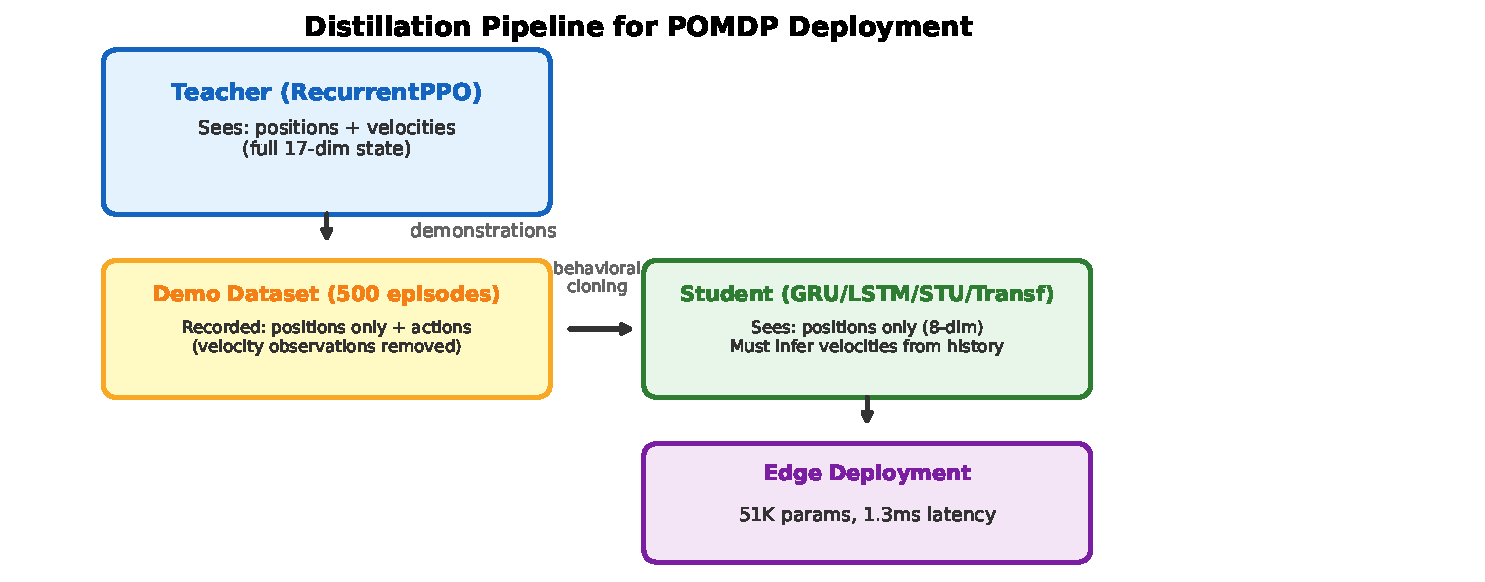
\includegraphics[width=0.8\textwidth]{diagram_pipeline.pdf}
\caption{Distillation pipeline. The teacher trains on full observations (positions + velocities), but demonstrations are recorded with only position observations. The student learns to map position histories to actions via behavioral cloning, then deploys on edge hardware.}
\label{fig:pipeline}
\end{figure}

Random baselines: HalfCheetah-POMDP $= -275 \pm 72$; Ant-POMDP $= -69 \pm 109$.

\section{Teacher Quality Manipulation}
\label{sec:teacher-quality}

We vary teacher quality along two axes:

\paragraph{Training progress.} Checkpoints at 200K, 500K, 1M, and 2M training timesteps.
\paragraph{Action noise.} Gaussian noise $\sigma \in \{0.0, 0.3\}$ added to actions during demonstration collection.

Together, these produce 8 teacher quality levels per environment, spanning returns from 210 to 1{,}424 (Ant) and 464 to 1{,}385 (HalfCheetah).

\begin{table}[ht]
\centering
\caption{Teacher return at each quality level (seed 42).}
\label{tab:teacher-quality}
\begin{tabular}{lcc}
\toprule
Teacher Configuration & HalfCheetah & Ant \\
\midrule
200K steps            & 534 & 647 \\
500K steps            & 1{,}013 & 963 \\
1M steps              & 1{,}385 & 1{,}424 \\
2M steps              & 1{,}378 & $439^*$ \\
\midrule
200K + noise $\sigma{=}0.3$ & 464 & 216 \\
500K + noise $\sigma{=}0.3$ & 592 & 251 \\
1M + noise $\sigma{=}0.3$   & 738 & 317 \\
2M + noise $\sigma{=}0.3$   & 811 & 210 \\
\bottomrule
\end{tabular}
\\[4pt]
{\small $^*$Ant teacher at 2M steps exhibits training instability.}
\end{table}

\section{Distillation Protocol}
\label{sec:distill-protocol}

For each (environment, teacher quality, student architecture, seed):
(1) collect 500 teacher episodes;
(2) split 80/20 train/val;
(3) train with MSE action loss (\cref{eq:bc}), AdamW lr${=}3{\times}10^{-4}$, cosine schedule, 100 epochs with early stopping (patience 10), gradient clipping at 1.0;
(4) evaluate: 20 rollouts in the POMDP.
We use 3 seeds (42, 123, 456) per condition; on four key conditions per environment, we run 2 additional seeds (789, 1337) for 5-seed estimates.

\section{JEPA Auxiliary Loss}
\label{sec:jepa-setup}

In addition to the action loss, we test a JEPA-style predictive latent auxiliary objective inspired by I-JEPA~\citep{assran2023ijepa} and V-JEPA~\citep{bardes2024vjepa}.
A predictor MLP takes the student's current hidden state $h_t$ and the next $k$ actions, and predicts the teacher's hidden state $k$ steps in the future:
\begin{equation}
  \loss_\text{JEPA} = \frac{1}{T-k} \sum_{t=1}^{T-k} \| f_\text{pred}(h_t, a_{t:t+k-1}) - \text{sg}(z_{t+k}^\text{teacher}) \|_2^2
\end{equation}
where $\text{sg}(\cdot)$ denotes stop-gradient and $k=5$.
The total objective is $\loss_\text{total} = \alpha \cdot \loss_\text{action} + \beta \cdot \loss_\text{hidden} + \delta \cdot \loss_\text{JEPA}$ with $\alpha=1.0$, $\beta=0.5$, $\delta \in \{0.0, 0.5\}$.
